
%(BEGIN_QUESTION)
% Copyright 2006, Tony R. Kuphaldt, released under the Creative Commons Attribution License (v 1.0)
% This means you may do almost anything with this work of mine, so long as you give me proper credit

Hobbybyggere av Tesla-spoler må ofte lage egne høyspenningskondensatorer for LC-resonanskretsen, som er kjernen i spolen:

$$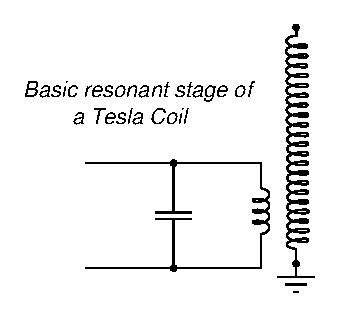
\includegraphics[width=15.5cm]{i00317x01.eps}$$

En kreativ måte å bygge slike kondensatorer på er å bruke gamle glassflasker fylt med saltvann, med metallstang eller kjetting ned i vannet, og aluminiumsfolie stramt rundt utsiden:

$$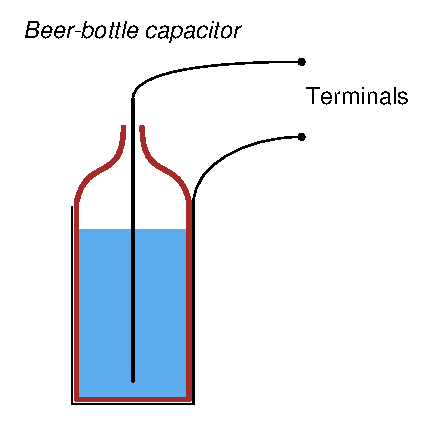
\includegraphics[width=15.5cm]{i00317x02.eps}$$

For å få nok kapasitans må man vanligvis koble flere slike flaskekondensatorer i parallell.  Poenget med flaskekondensatorer er jo nesten at man kan lage en ``sekspakning'' av dem.

\vskip 10pt

Så rart det enn virker, dette har faktisk en kobling til industriell instrumentering.  Identifiser hvilke deler av ``flaskekondensatoren'' som utgjør ledende plater i kondensatoren, og hvilken del som er dielektrikum.  Beskriv så hvordan kapasitansen påvirkes hvis nivået av saltvann i flasken endres.  Forklar til slutt hvordan dette prinsippet kan brukes til måling av væskenivå i en tank.

\vskip 20pt \vbox{\hrule \hbox{\strut \vrule{} {\bf Forslag til sokratisk diskusjon} \vrule} \hrule}

\begin{itemize}
\item{} Hvorfor brukes saltvann i stedet for vanlig springvann?
\item{} Hvis flasken hadde tynnere glass (alt annet likt), ville kapasitansen {\it øke} eller {\it minke}?
\item{} Hvis flasken var høyere (alt annet likt), ville kapasitansen {\it øke} eller {\it minke}?
\item{} Hvis flasken hadde større diameter (alt annet likt), ville kapasitansen {\it øke} eller {\it minke}?
\end{itemize}

\underbar{file i00317}
%(END_QUESTION)





%(BEGIN_ANSWER)

%(END_ANSWER)





%(BEGIN_NOTES)

Folien og vannet danner platene, mens glasset er dielektrikumet.  Kapasitansen øker når saltvannsnivået øker.

\vskip 10pt

Kapasitansformel:

$$C = {{A \epsilon} \over d}$$

\noindent
Der,

$C =$ Kapasitans i farad

$\epsilon =$ Permittivitet i dielektrikum (absolutt)

$A =$ Lederareal i kvadratmeter

$d =$ Avstand mellom lederne i meter

\vskip 10pt

\begin{itemize}
\item{} Flaske med tynnere glass (alt annet likt) -- kapasitans vil {\bf øke} (fordi $d$ blir mindre)
\item{} Høyere flaske (alt annet likt) -- kapasitans vil {\bf øke} (fordi $A$ blir større)
\item{} Flaske med større diameter (alt annet likt) -- kapasitans vil {\bf øke} (fordi $A$ blir større)
\end{itemize}

%INDEX% Measurement, level: capacitance

%(END_NOTES)
